%\subsection{Components}
%The components required for this manual are listed in Table \ref{table:components}
%\input{./figs/components.tex}
\subsection{Software Setup}
The following commands will install the Wiring Pi module
\begin{lstlisting}
git clone https://github.com/WiringPi/WiringPi.git
cd WiringPi && ./build
./build
cp blink.c ~
cd ~
\end{lstlisting}
Connect the Wiring Pi GPIO Pin 0 to an LED according to the pin diagram in 

\begin{lstlisting}
https://pinout.xyz/
\end{lstlisting}

\begin{lstlisting}
gcc -Wall -o test blink.c -lwiringPi
sudo ./test
\end{lstlisting}

%\subsection{Powering the Display}
%The breadboard can be divided into 5 segments.  In each of the green segements, the pins are internally connected so as to have the same voltage.  Similarly, in the central segments, the pins in each column  are internally connected in the same fashion as the blue columns. 
%
%\begin{problem}
%	Plug the display to the breadboard in Fig. \ref{fig:breadboard}
%\end{problem}
%\begin{figure}[!h]
%\begin{center}
%\includegraphics[width=\columnwidth]{./figs/breadboard}
%\end{center}
%\caption{}
%\label{fig:breadboard}
%\end{figure}
%
%The seven segment display in Fig. \ref{fig:sevenseg} has eight pins, $a, b, c, d, e, f, g$ and $dot$ that take an active LOW input, i.e.  the LED will glow only if the input is connected to ground.  Each of these pins is connected to an LED segment.  The $dot$ pin is  reserved for the $\cdot$ LED.  
%
%%
%%\begin{center}
%	%\includegraphics[scale=1]{sevenseg}
%%\end{center}
%
%\begin{problem}
%	Connect one end of the resistor to the COM pin of the display and the other end to an extreme pin of the breadboard.	
%\end{problem}
%%
%%
%%\begin{figure}[!h]
%%\begin{center}
%%\resizebox {0.5\columnwidth} {!} {
%%\input{./figs/sevenseg.tex}
%%}
%%\end{center}
%%\caption{}
%%\label{fig:sevenseg}
%%\end{figure}
%
%The Raspberry Pi 3 has 40 pins (see Figs. \ref{fig_1_3a} and \ref{fig_1_3b}), which include power pins that can generate 5V and 3.3V, GND pins, PWM pins, pins for wired communication and some free pins for digital I/O.  In the following exercises, only the GND, 5$V$ and digital I/O pins will be used.
%
%%Arduino Uno has some ground pins, analog input pins A0-A3 and digital pins D1-D13 that can be used for both input as well as output. It also has two power pins that can generate 3.3$V$ and 5$V$.  In the following exercises, only the GND, 5$V$ and digital pins will be used.
%%
%%\begin{center}
%	%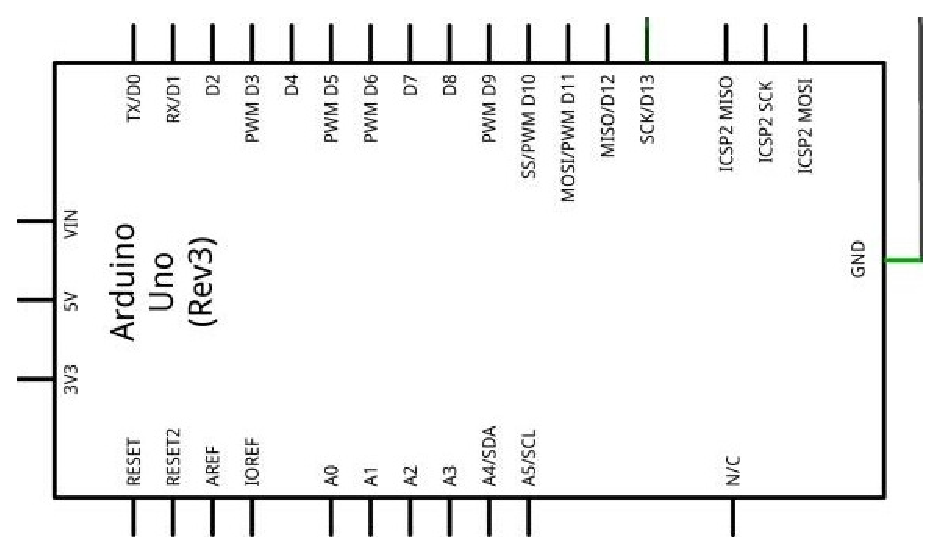
\includegraphics[scale=1]{arduino}
%%\end{center}
%%
%\begin{problem}
%	Connect pin 2 (5V) of the Pi to an  extreme pin that is in the same segment as the resistor pin. 
%	\end{problem}	
%\begin{problem}
%	Connect pin 6 (GND) of the Pi to the opposite extreme pin of the breadboard
%\end{problem}
%%\begin{problem}
%%	Connect the Arduino to the computer.
%%\end{problem}
%\begin{problem}
%	Connect the \em{dot} pin of the display to a pin in the same segment as the GND pin.  What do you observe?
%\end{problem}
%\subsection{Controlling the Display}
%Fig. \ref{fig:sevenseg12} explains how to get decimal digits using the seven segment display. 
%\begin{problem}
%	Generate the number 1 on the display by connecting only the pins $b$ and $c$ to GND. 
%\end{problem}	
%%
%\begin{figure}[!h]
%\begin{center}
%\resizebox {0.8\columnwidth} {!} {
%\input{./figs/sevenseg12.tex}
%}
%\end{center}
%\caption{}
%\label{fig:sevenseg12}
%\end{figure}
%
%\begin{problem}
%	Repeat the above exercise to generate the number 2 on the display.
%\end{problem}	
%%
%\renewcommand{\thetable}{\theproblem}
%\begin{problem}
%Table \ref{table:arduioport} summarizes the process of generating the decimal digits.  0 means connecting to ground and 1 means not connecting.  	Complete Table \ref{table:arduioport} for all numbers between 0-9.
%\end{problem}	
%\input{./figs/arduinoport}
%%
%%
%\begin{problem}
%	Now generate all numbers between  0-9 on the display using the above table.
%\end{problem}
